\documentclass[tikz]{standalone}

\usepackage[T2A]{fontenc}
\usepackage[utf8x]{inputenc}
\usepackage{amsmath,amssymb}
\usepackage{cmap,pgfplots,pgfplotstable}
\pgfplotsset{compat=newest}
\usetikzlibrary{patterns}

\begin{document}
% \pgfplotstableread{data.tsv}\mytable 
	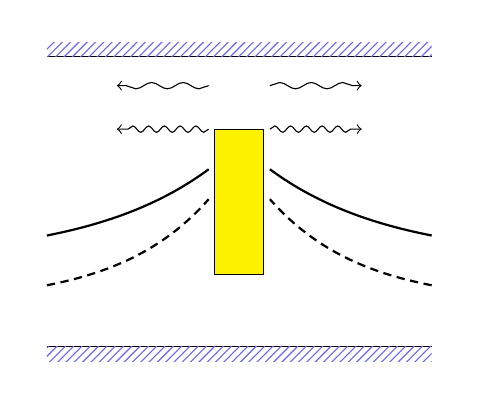
\begin{tikzpicture}[
	    interface1/.style={
        % The border decoration is a path replacing decorator. 
        % For the interface style we want to draw the original path.
        % The postaction option is therefore used to ensure that the
        % border decoration is drawn *after* the original path.
        postaction={draw=blue,decorate,decoration={border,angle=-135,
                    amplitude=0.2cm,segment length=3mm}}}, 
    interface/.style={
        pattern = north east lines,
        draw    = none,
        pattern color=blue!60,          
    },
		]
		\begin{axis}[
			% width=7cm,
			height=6 cm,
			% enlargelimits = true,
			% legend pos= south east,
			legend pos=outer north east,
			ymax = 1.2,
			ymin = -1.2,
			xmax = 1.1*pi,
			xmin = -1.1*pi,
			% scale=1,
			% ylabel={$\mathrm{Re}\,E_x$}, 			% подпись оси Y
			% xlabel={$z$}, 			% подпись оси X
			% xticklabels={},
				% yticklabels={},
			xtick=\empty,
			ytick=\empty,
			%major grid style={
			%	line width=0.5pt, 	% толщина основных линий сетки
			%	draw=black!50 		% цвет основных линий сетки: 50% черного (80% белого) 
			%},
			minor grid style={
				line width=0.5pt, 	% толщина промежуточных линий сетки
				draw=black!20		% цвет промежуточных линий сетки
			},
			%minor tick num=1,		% количество промежуточных линий между основными
 			ticklabel style={
 				% scale=0.1			% уменьшим размер подписей меток на осях
 			},    
 			%xticklabel style={above, yshift=0.25em},
 			%yticklabel style={right},
	    	axis lines=middle, 		% выравнивание оси y:  middle (в нуле)|left|right
			%enlargelimits=true,
			%xtick distance=0.5,		% расстояние между метками по оси X
			%ytick distance=0.5,		% расстояние между метками по оси Y
			% unit vector ratio = 1 1,% масштаб 1:1 осей X и Y
			% clip=false,
			% ymax= 1.5,
    		x label style={
    		at={(current axis.right of origin)}, 
            xshift=1.7ex, anchor=center
    		},
    		y axis line style={draw=none,},
    		x axis line style={draw=none,},
% extra x ticks={1},	% положение дополнительных тиков
% extra x tick labels={	% их подписи
 		% {$\omega_{cr_{n}}$}
% }, 		
    		y label style={
    			% at={(axis description cs:0.01,1.07)},
    			draw=none,
    			yshift=0.7em,
    			anchor=center,		% расПоложение метКи ровно в точКе (0,1.1)
    			% black				% цвет метКи
    		},		
		]

		\addplot[thick,domain={-pi:-1/2},samples=350] {exp(+x/2)*0.8-0.4};
		\addplot[thick,domain={pi:1/2},samples=350] {exp(-x/2)*0.8-0.4};
		\addplot[thick,densely dashed,domain={-pi:-1/2},samples=350] {exp(+x/1.5)-0.7};
		\addplot[thick,densely dashed,domain={pi:1/2},samples=350] {exp(-x/1.5)-0.7};

		% \foreach \dd in {0.2,-0.2,-0.6,-1}{
		% 	\addplot[thick,dashed, opacity=0.6,domain={-pi:1},samples=350] {exp(+x/2)/2*\dd};
		% }


		\draw[black] (-pi,-1) -- (pi,-1);
		\draw[black] (pi,1) -- (-pi,1);

		\draw[interface] (-pi,-1) rectangle (pi,-1-0.1);
		\draw[interface] (pi,1)  rectangle (-pi,1+0.1);

		\draw[fill=yellow] (-1/2.5,-1/2) rectangle (1/2.5,1/2);

		\draw [->,decorate,decoration={snake,amplitude=.4mm,segment length=2mm,post length=1mm}] 		(1/2,1/2) -- (2,1/2);
		\draw [->,decorate,decoration={snake,amplitude=.4mm,segment length=4mm,post length=1mm}] 		(1/2,1/2+0.3) -- (2,1/2+0.3);
		
		\draw [->,decorate,decoration={snake,amplitude=.4mm,segment length=2mm,post length=1mm}] 		(-1/2,1/2) -- (-2,1/2);
		\draw [->,decorate,decoration={snake,amplitude=.4mm,segment length=4mm,post length=1mm}] 		(-1/2,1/2+0.3) -- (-2,1/2+0.3);

		% \draw (pi/2,1/2) node [above] {$h>0:\,\, \longrightarrow$};
		% \addplot[thick,domain={0:1},samples=100] {0};
		% Добавляем графики на рисунок
		% \addplot[smooth] table[x expr=\thisrow{xi}, y expr=\thisrow{E0}] {\mytable};
		% \addplot[smooth] table[x expr=\thisrow{xi}, y expr=\thisrow{E1}] {\mytable};
		% \addplot[smooth] table[x expr=\thisrow{xi}, y expr=\thisrow{E2}] {\mytable};
		% \addplot[smooth] table[x expr=\thisrow{xi}, y expr=\thisrow{E3}] {\mytable};
		% \addplot[smooth] table[x expr=\thisrow{xi}, y expr=\thisrow{E4}] {\mytable};

		% \addplot[smooth, dashed] table[x expr=\thisrow{xi}, y expr=\thisrow{E0n}] {\mytable};
		% \addplot[smooth, dashed] table[x expr=\thisrow{xi}, y expr=\thisrow{E1n}] {\mytable};
		% \addplot[smooth, dashed] table[x expr=\thisrow{xi}, y expr=\thisrow{E2n}] {\mytable};
		% \addplot[smooth, dashed] table[x expr=\thisrow{xi}, y expr=\thisrow{E3n}] {\mytable};
		% \addplot[smooth, dashed] table[x expr=\thisrow{xi}, y expr=\thisrow{E4n}] {\mytable};
		
       	\end{axis}
	\end{tikzpicture}	
\end{document}